\chapter{Simulation Design}
\section{Choice of Software}
The simulation environment was created using MATLAB and Simulink. MATLAB provides a comprehensive environment, with support for packages such as the UAV Toolbox, for simulating UAVs. MATLAB also has support for Path Planning and Navigation Toolboxes for generating flight trajectories and an Autopilot and Control Systems Toolbox for designing and analysing a controller. Another key advantage to MATLAB and Simulink is the integration and support for ANFIS controllers. This will allow development of our ANFIS controller in the same environment as our simulator, easing development. 

The simulator was heavily adapted from an existing example on UAV Obstacle Avoidance from Simulink. By modifying and adding our own elements to the Simulink programme, a bespoke solution for data collection was achieved. Autonomous scenarios and drone control allowed for data collection without the need for manual input, saving a large amount of time, and allowed for concurrent simulations to run, increasing the amount of data collected.
\section{Simulink Structure}
The developed Simulink model is shown in Figure \ref{fig:sim1} and is based on a model from MathWorks. Many different ``blocks'' can be seen, divided into three main sections:
\begin{itemize}
    \item UAV Scenario
    \begin{itemize}
        \item UAV Scenarios Motion Read: captures current UAV state
        \item UAV Scenario LIDAR: captures LIDAR sensor data
        \item UAV Scenario Scope: visualisation of trajectory and LIDAR data
        \item UAV Scenario Configuration: configuration of scenario
        \item UAV Scenario Motion Write: updates UAV state
    \end{itemize}
    \item Waypoint following and obstacle avoidance
    \begin{itemize}
        \item Waypoint Follower: computes a lookahead point for the UAV
        \item Obstacle Avoidance: 3D VFH+ algorithm is used to calculate a safe direction and yaw for unobstructed flight, updating the Waypoint Follower block's lookahead point accordingly
        \item Enable Obstacle Avoidance: enable or disable obstacle avoidance
    \end{itemize}
    \item Controller and plant
    \begin{itemize}
        \item Controller: responsible for generating control signals for the UAV
        \item Quadrotor Plant: updates UAV state with control signal
    \end{itemize}
\end{itemize}
These concepts are explained in detail in later sections.
\begin{figure}[H]
    \centering
    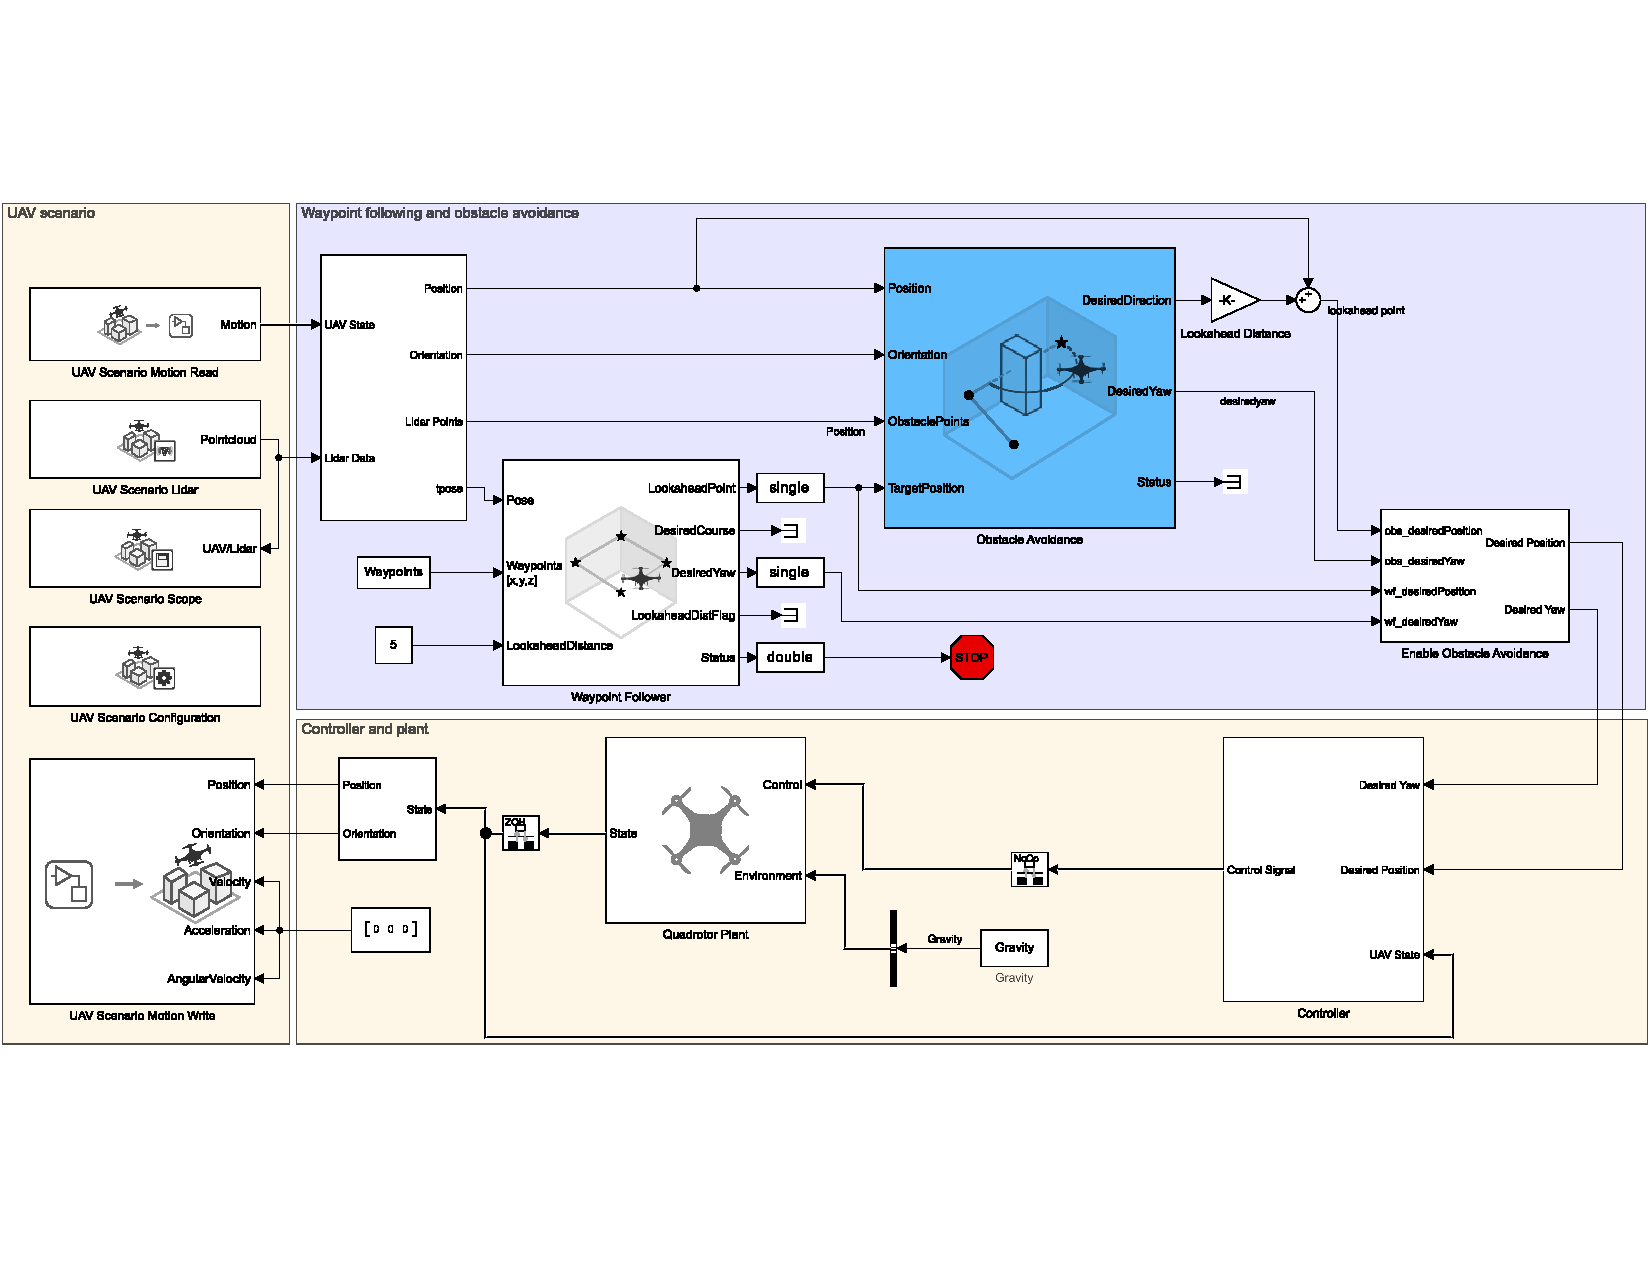
\includegraphics[width =\textwidth]{img/simulink_model.pdf}
    \caption{Simulink model.}
    \label{fig:sim1}
\end{figure}
A key addition for the data collection was the addition of random scenario generation to the model. Further, for the data collection, some of the parameters and function of the blocks in the diagram above were re-coded. The significant change to the simulation is the waypoints and obstacles generation. In the original Simulink process and code, the waypoints and the obstacles were fixed. Hence, a new function code was required in order to replace the fixed waypoints generator. Random waypoint generation is crucial to allow for a range of scenarios and motions to be recorded during simulation. This is to capture as much of the drone dynamics as possible, in order to train the fuzzy inference system with a wide and robust set of data.
\subsection{Quadrotor Model}
The quadrotor model used in this project is a generic commercial quadrotor. A commercial quadrotor such as a DJI drone is highly versatile and has all the specifications available. Also, using a commercial model means that the results of the simulation are representative of real-world use. Additionally, the cost of the quadrotor is likely to be lower than educational products. A complete set of sensors is also installed. Therefore, the commercial quadrotor is the best option in this case.

The quadrotor used in the simulation has mass \SI{1}{kg} and radius \SI{10}{cm}. These values are representative of a generic small-to-medium-sized quadrotor. The quadrotor model in the simulator uses a reduced-order guidance block. This block uses a closed-loop system, which includes the UAV dynamics and autopilot. It is used for small multi-rotor UAVs. Although this may not be the most realistic nor accurate model, as it is reduced order, it provided results which can be easily used and extracted. The autopilot gains are kept the same as in the original model. The following equations govern the quadrotor model. The position of the UAV in the world frame is:
\begin{equation}
    \begin{bmatrix} x & y & z\end{bmatrix}
\end{equation}
The orientation, roll, pitch, and yaw, is: 
\begin{equation}
    \begin{bmatrix} \phi & \theta & \psi\end{bmatrix}
\end{equation}
The respective angular velocities are: 
\begin{equation}
    \begin{bmatrix} p & q & r\end{bmatrix}
\end{equation}
The model takes a commanded roll, pitch, yaw rate, and total thrust:
\begin{equation}
    \begin{bmatrix} \phi^{Control} & \theta^{Control} & \dot{\psi}^{Control} & F^{Control}_{thrust}\end{bmatrix}
\end{equation}
The outputs are the position, velocities, orientation, angular velocities, and thrust:
\begin{equation}
\setcounter{MaxMatrixCols}{20}
    \begin{bmatrix} x & y & z & \dot{x} & \dot{y} & \dot{z} & \phi & \theta & \psi & p & q & r & F_{thrust} \end{bmatrix}
\end{equation}
The rotation matrix $R$ is given by:
\begin{equation}\label{rotation matrix}
R=
\begin{bmatrix}
\cos{\theta}\cos{\psi} & \cos{\psi}\sin{\phi}\sin{\theta}-\cos{\phi}\sin{\psi} & \cos{\psi}\cos{\phi}\sin{\theta}+\sin{\phi}\sin{\psi}\\
\cos{\theta}\sin{\psi} & \cos{\phi}\cos{\psi}+\sin{\phi}\sin{\psi}\sin{\theta} & -\sin{\phi}\cos{\psi}+\cos{\phi}\sin{\psi}\sin{\theta}\\
-\sin{\theta} & \cos{\theta}\sin{\phi} & \cos{\theta}\cos{\phi}
\end{bmatrix}
\end{equation}
The acceleration of the drone is given by:
\begin{equation}\label{drone accel}
m
\begin{bmatrix}
\ddot{x}\\
\ddot{y}\\
\ddot{z}
\end{bmatrix}
=
\begin{bmatrix}
0\\
0\\
mg
\end{bmatrix}
+ R
\begin{bmatrix}
0\\
0\\
-F_{thrust}
\end{bmatrix}
\end{equation}
where $m$ is the mass of the drone and $g$ is the acceleration due to gravity. The angular velocities are given by:
\begin{equation}\label{angular velocity}
\begin{bmatrix}
\dot{\phi}\\
\dot{\theta}\\
\dot{\psi}
\end{bmatrix}
=
\begin{bmatrix}
1 & \sin{\phi}\tan{\theta} & \cos{\phi}\tan{\theta}\\
0 & \cos{\phi} & -\sin{\phi}\\
0 & \dfrac{\sin{\phi}}{\cos{\theta}} & \dfrac{\cos{\phi}}{\cos{\theta}}
\end{bmatrix}
\begin{bmatrix}
p\\
q\\
r
\end{bmatrix}
\end{equation}
The block approximates a closed-loop controller for the roll, pitch, yaw rate, and thrust. Roll and pitch are controlled using a PD controller, while yaw rate and thrust are controlled using a P controller. The angular accelerations are given by:
\begin{equation}\label{angular accel}
\begin{bmatrix}
\dot{p}\\
\dot{q}\\
\dot{r}
\end{bmatrix}
=
\begin{bmatrix}
1 & 0 & -\sin{\theta}\\
0 & \cos{\phi} & \sin{\phi}\cos{\theta}\\
0 & -\sin{\phi} & \cos{\phi}\cos{\theta}
\end{bmatrix}
\begin{bmatrix}
KP_\phi(\phi^{Control}-\phi)+KD_\phi(-\dot{\phi})\\
KP_\theta(\theta^{Control}-\theta)+KD_\theta(-\dot{\theta})\\
KP_\psi(\dot{\psi}^{Control}-\dot{\psi})
\end{bmatrix}
\end{equation}
where $KP$ and $KD$ are the proportional and derivative gains. The thrust rate is given by:
\begin{equation}\label{thrust eqn}
\dot{F}_{thrust}=KP_F(F^{Control}_{thrust}-F_{thrust})
\end{equation}
\subsection{Sensors}
The LIDAR sensor sends rapid laser pulses, which are reflected off objects, and receives the response to map out an area. This allows for path planning and obstacle avoidance algorithms to work as it provides a map of the environment in its vicinity. LIDAR creates a point cloud based on the points that the laser reflects back to the sensing unit. This provides information on the distances of each point of the obstacle, mapping the drone’s surroundings.

An alternative for LIDAR is using cameras for photogrammetry systems. Although cameras are cheap, LIDAR has the advantage of being able to works at any time of the day, while cameras may not be able to provide sufficient detail in the dark. Additionally, cameras require high processing capabilities \cite{9278591}.  

Table \ref{tab:zain3} shows the LIDAR sensing unit’s parameters, set to standard ranges given by MathWorks. 
\begin{table}[H]
    \centering
    \begin{tabular}{@{}ll@{}}
        \toprule
        \textbf{Parameter} & \textbf{Value(s)}\\
        \midrule
        Maximum range & \SI{7}{\meter}\\
        Range accuracy & \SI{0.02}{\meter}\\
        Azimuthal limits & \SI{-179}{\degree} to \SI{179}{\degree}\\
        Elevation limits & \SI{-15}{\degree} to \SI{15}{\degree}\\
        Azimuthal resolution & \SI{0.5}{\degree}\\
        Elevation resolution & \SI{2}{\degree}\\
        Sample time & \SI{0.01}{\second}\\
        \bottomrule
    \end{tabular}
    \caption{LIDAR parameters.}
    \label{tab:zain3}
\end{table}
\subsection{Waypoint Following}
The Waypoint Follower block, shown in Figure \ref{fig:wp_follower}, is used to follow a set of waypoints using a lookahead distance, which determines the distance at which the target point - lookahead point - will be. It calculates the lookahead point, desired trajectory, and desired yaw. Its inputs are the current state (position and orientation), the waypoints, and the lookahead distance. Using this information, it calculates an intermediate point for the UAV to move towards, in order to reach the waypoints. The desired position and desired yaw data is crucial to building the neuro-fuzzy controller as these datapoints directly relate to the control signal applied to the drone.
\begin{itemize}
    \item \textbf{Position and Orientation:} The current position and orientation (roll, pitch, yaw) of the UAV.
    \item \textbf{Waypoints:} The coordinates of the waypoints.
    \item \textbf{Lookahead Point:} This is the desired point for the UAV to move to, in order to get closer to the next waypoint. In the setting of this parameter, a minimum and maximum distance are required, which are set as \SI{0.2}{\meter} and \SI{5}{\meter} respectively. The distance determines how far away the lookahead point will be. This output is fed to the Obstacle Avoidance Block.
\end{itemize} 
\begin{figure}[H]
    \centering
    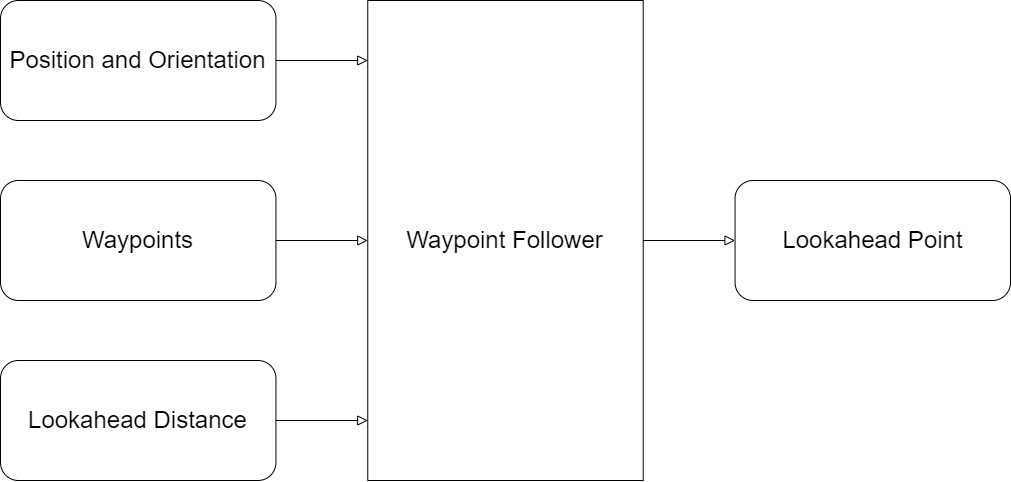
\includegraphics[width = 0.7\textwidth]{./img/wp_follower.png}
    \caption{Inputs and outputs of the Waypoint Follower block.}
    \label{fig:wp_follower}
\end{figure}
When following a set of waypoints, in this case, the drone will most likely ignore the first waypoint as the drone pose is set to start in hover or to start from the ground. The pose of a drone is a combination of its yaw, pitch and roll angle that the drone is actually performed \cite{Roy5}. The initial yaw, pitch and roll angle are zero. Depending on the drone's heading, the drone will try to start from the current waypoint to the next one in a linear path although in a realistic scenario, the drone has to constantly change its heading to stabilise. The pitch, yaw or roll angle is changed, which depends on the difference of altitude and heading between two defined waypoints. In this simulation, paths between each waypoints, including the initial path, are being split into different path segments. In most cases, the drone is driven by the control signal in order to track the path segments. In the second condition, a transition region is introduced in order to smooth the path taken. Based on the nature of the lookahead distance for path tracking, if the quadrotor is within \SI{0.1}{\meter} to the next waypoint, the transition region is used. In the third condition, the lookahead distance is not in the transition region but the drone's heading is about to change. In this case, a 3D hyperplane is drawn at the next waypoint. 

From documentation from Mathworks, a hyperplane is the vector space that is contained in the current space. If the current space is a $n$ dimensional space or vector, the hyperplane of this space or vector will be a $n-1$ dimensional space or vector. For example, on a 2D surface, the hyperplane is a line on the surface. Equivalently, in a 3D space, the hyperplane is a surface inside of this volume. Figure \ref{fig:hyperplane} shows the transition region of the waypoint and the hyperplane region in top view. Once the drone is inside of the hyperplane, the waypoints follower directs the quadrotor from the current waypoint to the next waypoint. One of the boundaries of the hyperplane is perpendicular to the direct path from last waypoint and the next waypoint and it is parallel to the ground surface. This smooths the trajectory to the next waypoint and allows for a more stable flight path. The hyperplane condition is defined by the following equations,
\begin{gather}
    \left(p - w_1 \right)^T\left(w_2 - w_1\right) \geq 0
\end{gather}
where $p$ is the position of the quadrotor, $w_1$ and $w_2$ are sequential waypoint positions. The vector $p$, $w_1$ and $w_2$ has three components, ($x$, $y$, $z$). $T$ represents the transpose of the matrix. $p_1$ is the first scenario that the drone is not in the hyperplane. The red line $p_1$ represents the lookahead distance that is set before the simulation starts. Once the lookahead distance enters into the transition region, the drone starts to turn onto the next path segment. Another scenario is $p_2$, where the drone is in the hyperplane region. In this case, the drone is changing its heading and moving onto the next path segment. The first part of the inequality ($p-w_1$) represents the vector of the displacement between the position of drone $p$ and the position of waypoint $w_1$. The second part of the inequality ($w_2-w_1$) is the vector of the displacement between the waypoint just passed and the next waypoint the drone is heading to. The result of their product is a number. When it less then zero, the specific hyperplane is not used. If the result is equal or larger to zero, the drone determines that it is located inside the hyperplane region. Therefore, the hyperplane condition is enabled.
\begin{figure}[H]
    \centering
    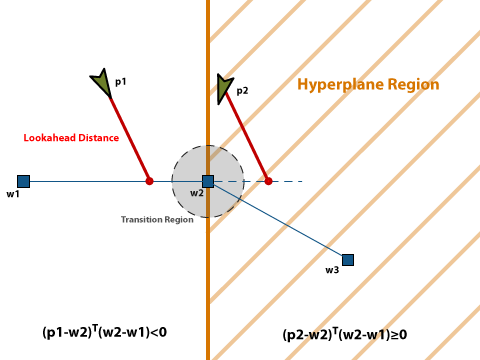
\includegraphics[width = 0.7\textwidth]{./img/fig9.png}
    \caption[Hyperplane illustration.]{Hyperplane illustration from MathWorks.}
    \label{fig:hyperplane}
\end{figure}
\subsection{Obstacle Avoidance}
The obstacle avoidance block from the UAV toolbox is used, a simplified diagram is shown in Figure \ref{fig:obs_avoid}. Obstacle avoidance is enabled through the use of a LIDAR sensor, which allows the algorithm to compute an obstacle-free direction towards a lookahead point, which is determined by the waypoints.
\begin{itemize}
    \item \textbf{Position and Orientation:} The current position and orientation (roll, pitch, yaw) of the UAV.
    \item \textbf{Obstacle Points:} These are obtained from the point cloud from the LIDAR sensor, indicating the points where an obstacle is detected.
    \item \textbf{Target Position:} This is the lookahead point from the Waypoint Follower Block.
    \item \textbf{Obstacle-Free Direction:} The desired direction of movement which does not have an obstacle.
    \item \textbf{Obstacle-Free Point:} The desired point of movement in the obstacle-free direction.
    \item \textbf{Desired Yaw:} The desired yaw in order to turn to the obstacle-free direction.
\end{itemize}
\begin{figure}[H]
    \centering
    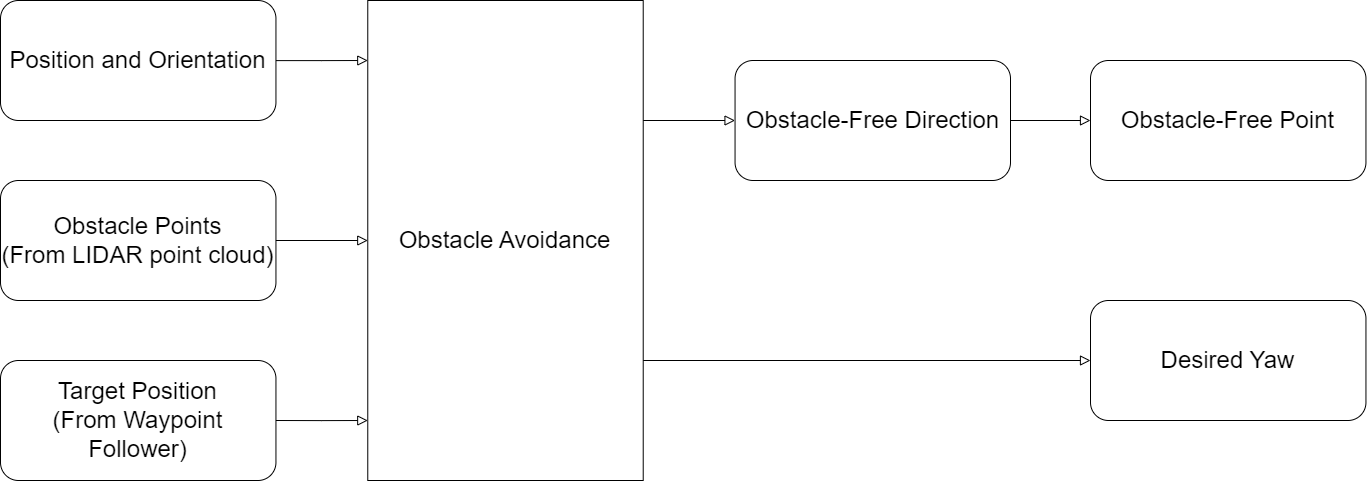
\includegraphics[width = 0.8\textwidth]{./img/obs_avoid.png}
    \caption{Simplified Obstacle Avoidance block.}
    \label{fig:obs_avoid}
\end{figure}
The inputs are the UAV state (position and orientation), the obstacle points, which are given by the LIDAR, and the target position, given by the Waypoint Follower Block as the lookahead point. This block computes a desired direction and yaw for the drone to move. This is then fed into the lookahead distance, which finds the furthest point in the desired direction where there is no obstacle. These are then fed into the controller.

A cost function is used determine the desired direction. This is defined using the target direction, current direction, previous direction, and their associated weights. The weights for these are 5, 2, 2 respectively. The highest weight is in the target direction, meaning deviating from the target direction will be penalised more heavily than the other directions. The block finds the minimum of the cost function to determine the desired direction and yaw for the drone.
\section{Simulation Environment}
The simulation environment is designed using random obstacle and waypoint generation, thereby allowing for a wide range of scenarios to be simulated. The map size is \SI{50}{\meter} $\times$ \SI{50}{\meter}. This is chosen to have a lower computational time, whilst still having a dense environment for the drone to navigate.

Three to four cuboid obstacles are generated with varying dimensions. This is to simulate a high density environment for the drone to navigate. The dimensions for the obstacles are chosen to be less than one-quarter of the map size, and represent various obstacles. For example, buildings are represented as obstacles with lengths and widths of greater than \SI{8}{\meter}, and small trees are represented as obstacles sized around \SI{1}{\meter} to \SI{3}{\meter}. The height is chosen to be up to around five storeys or \SI{20}{\meter}, to account for the varying height of buildings, trees, and other obstacles.

Three to six waypoints are generated randomly, represented as discs that are \SI{5}{\meter} below the actual waypoint position in the environment. This is done to prevent the drone from crashing into the discs, while still allowing for visualisation of the waypoints. This number of waypoints are chosen to allow the drone to navigate a large portion of the environment, thereby requiring more manoeuvres to be completed, for a rich dataset. The properties of the environment are shown in Table \ref{tab:zain5}.
\begin{table}[H]
    \centering
    \begin{tabular}{@{}ll@{}}
        \toprule
        \textbf{Parameter} & \textbf{Value(s)}\\
        \midrule
        Map Size & \SI{50}{\meter} $\times$ \SI{50}{\meter} \\
        Number of Waypoints & 3 to 6\\
        Number of Obstacles & 3 to 4 \\
        Obstacle Width & \SI{1}{\meter} to \SI{13}{\meter}\\
        Obstacle Length & \SI{1}{\meter} to \SI{13}{\meter}\\
        Obstacle Height & \SI{5}{\meter} to \SI{20}{\meter}\\
        \bottomrule
    \end{tabular}
    \caption{Simulation environment parameters.}
    \label{tab:zain5}
\end{table}
 A generated scenario is shown in Figure \ref{fig:sim_pic_5}. Two obstacle maps are created. One to check for any intersections between obstacles and waypoints, and another where the scenario will run. For the map used to check for intersections, the obstacles and waypoints have dimensions increased by \SI{1}{\meter} on each side of the lengths and widths. This ensures that in the real simulation map, there will be a minimum distance of \SI{2}{\meter} between obstacles, allowing the drone to move between obstacles.
\begin{figure}[H]
    \centering
    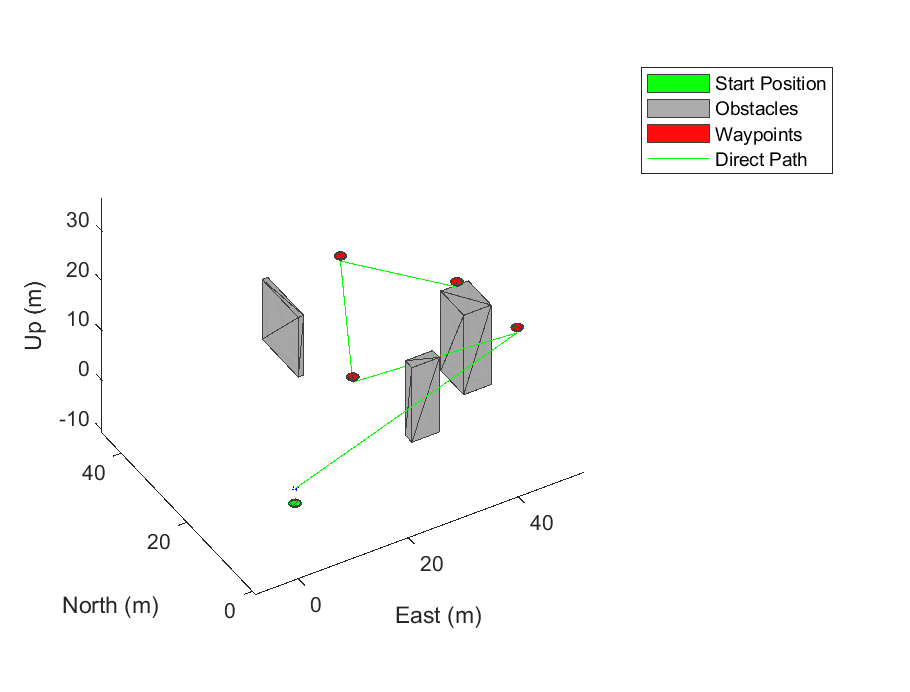
\includegraphics[width = 0.75\textwidth]{./img/sim_pic_5.eps}
    \caption{Randomly generated scenario.}
    \label{fig:sim_pic_5}
\end{figure}
In the simulator, the UAV will navigate to the next waypoint, in order, while moving to avoid any obstacles in its way. In a scenario where the waypoints are of the same height, such as in Figures \ref{fig:sim_pic_1} and \ref{fig:sim_pic_4}, it is able to simulate the flight of the quadrotor without colliding with obstacles. Additionally, the drone does not need to reach the exact location of the waypoint; it only needs to be within \SI{0.1}{\meter}, then it will move on to the next one, as seen in the same figure. The LIDAR sensing can be seen as a point cloud on the surface of an obstacle, seen in Figure \ref{fig:sim_pic_1} and Figure \ref{fig:sim_pic_4}, with the colour of each point indicating the distance away from the drone. This allows visualisation of what the drone can and cannot detect as it navigates through the environment, and enables obstacle avoidance.
\begin{figure}[H]
    \centering
    \begin{minipage}[b]{0.45\textwidth}
        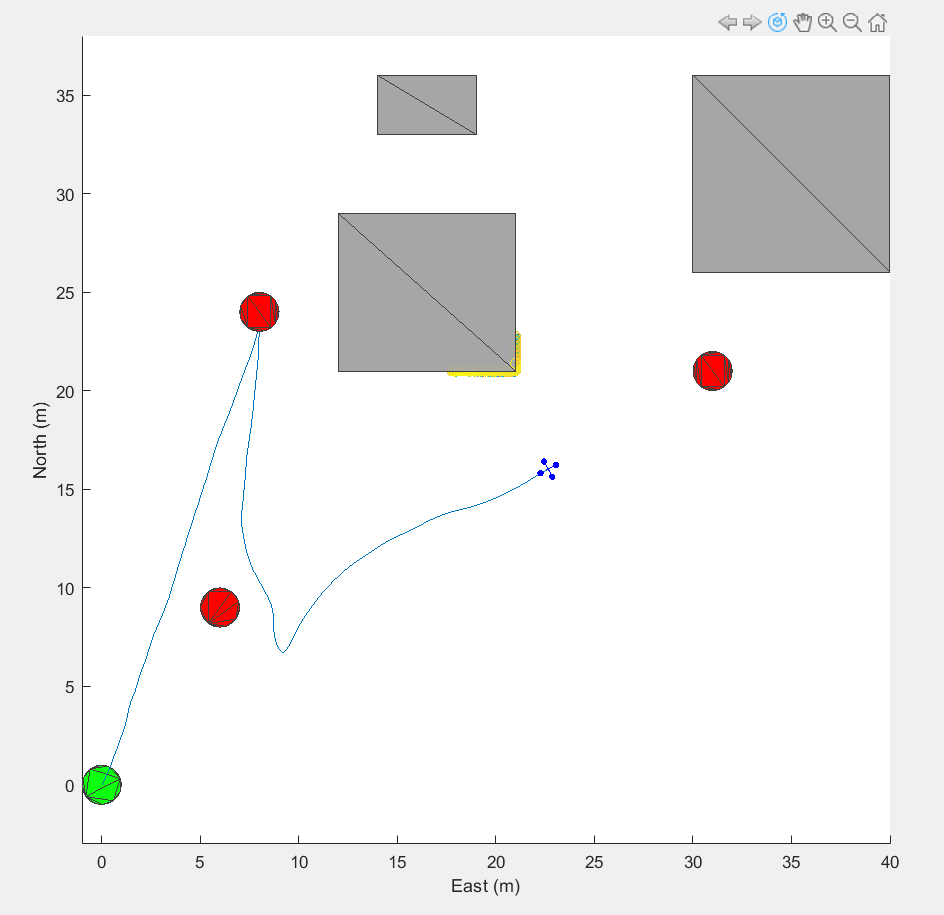
\includegraphics[height=7cm,keepaspectratio]{./img/sim_pic_1.png}
        \caption{Movement of drone in a random scenario with waypoints at the same height.}
        \label{fig:sim_pic_1}
    \end{minipage}
    \hfill
    \begin{minipage}[b]{0.45\textwidth}
        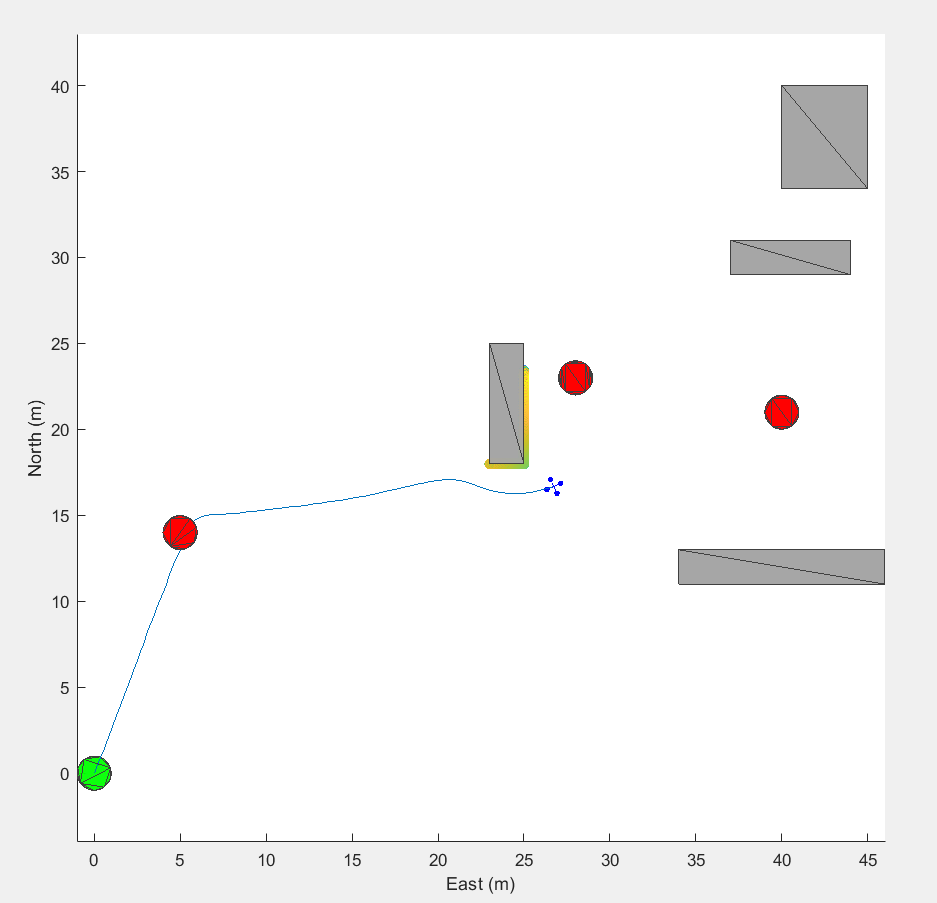
\includegraphics[height=7cm,keepaspectratio]{./img/sim_pic_4.png}
        \caption{Movement of drone in typical scenario. Point cloud on can be seen on obstacle near the drone.}
        \label{fig:sim_pic_4}
    \end{minipage}
\end{figure}
In scenarios where the waypoints differ in height, the behaviour of the drone changes. This is shown in Figure \ref{fig:sim_pic_2}. When ascending or descending, the drone moves in a spiral motion. This may be due to the LIDAR not being able to detect vertically upwards and downwards; therefore the drone attempts to spiral instead of moving vertically. This can be seen in Figure \ref{fig:sim_pic_3}.
\begin{figure}[H]
    \centering
    \begin{minipage}[b]{0.45\textwidth}
        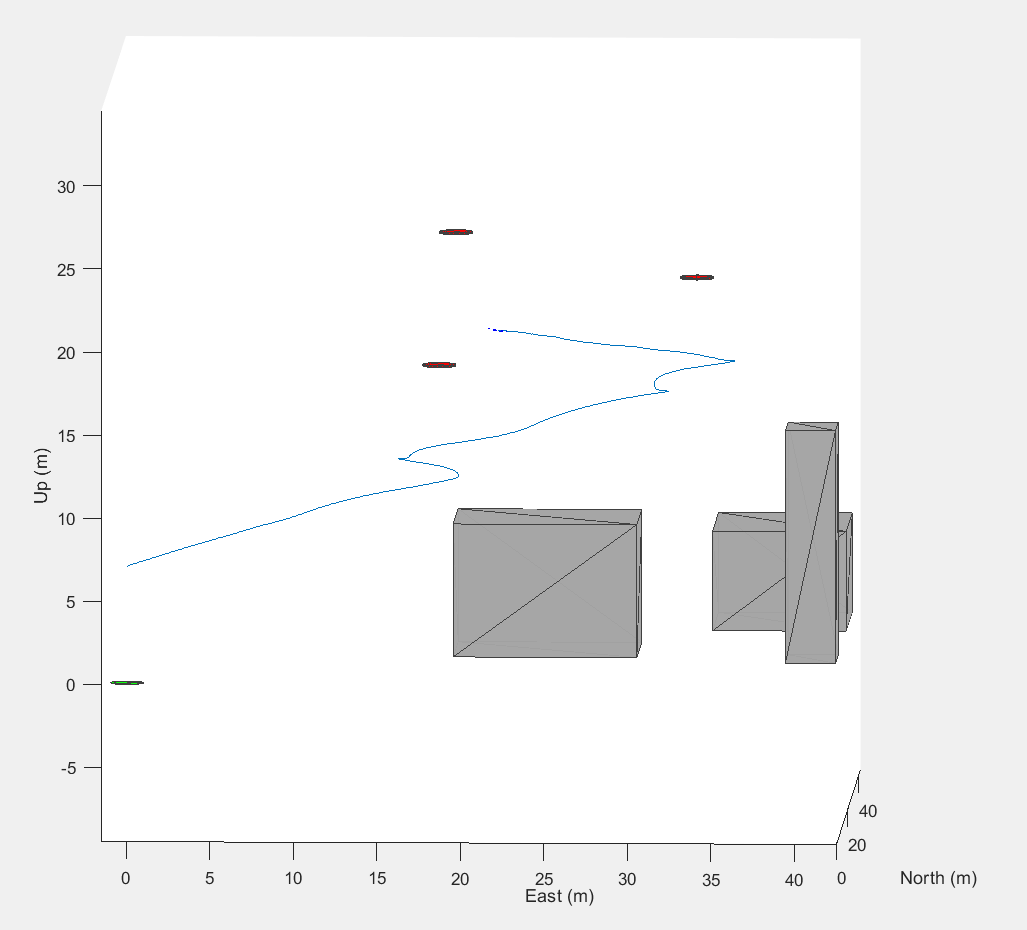
\includegraphics[height=7cm,keepaspectratio]{./img/sim_pic_2.png}
        \caption{Movement of drone in a random scenario with waypoints at the different heights.}
        \label{fig:sim_pic_2}
    \end{minipage}
    \hfill
    \begin{minipage}[b]{0.45\textwidth}
        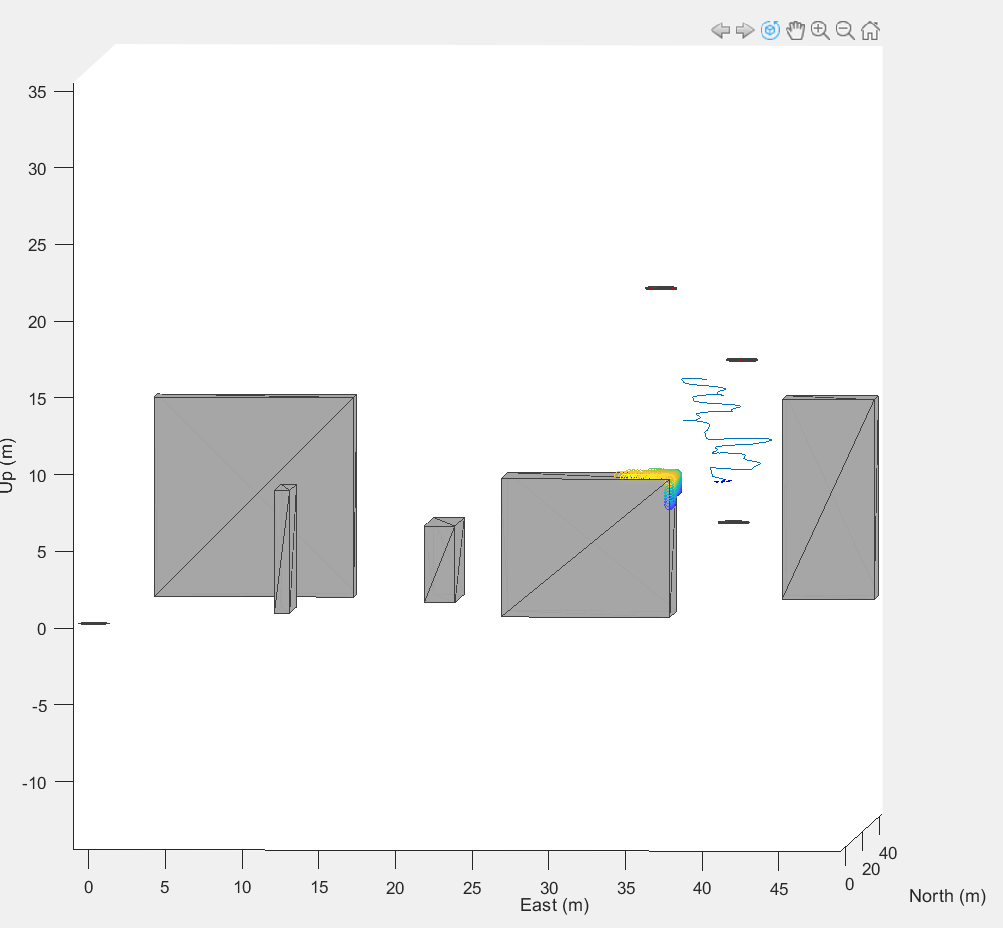
\includegraphics[height=7cm,keepaspectratio]{./img/sim_pic_3.png}
        \caption{Spiralling path of drone as drone descends.}
        \label{fig:sim_pic_3}
    \end{minipage}
\end{figure}

\section{Scenarios}
Five scenarios are created to compare the FIS controller and PID controller. These aim to put the drone in different environments, such as in open air without obstacles, or in urban environments where the drone must navigate through buildings.

\subsection{Scenario 1}
The first scenario is shown in Figure \ref{fig:3_3_scenario1}. It does not have any obstacles, to test the controller in an open air environment. This scenario aims to test the controller in navigating waypoints of different heights with a small turn, without any obstacle avoidance. 
\begin{figure}[H]
    \centering
    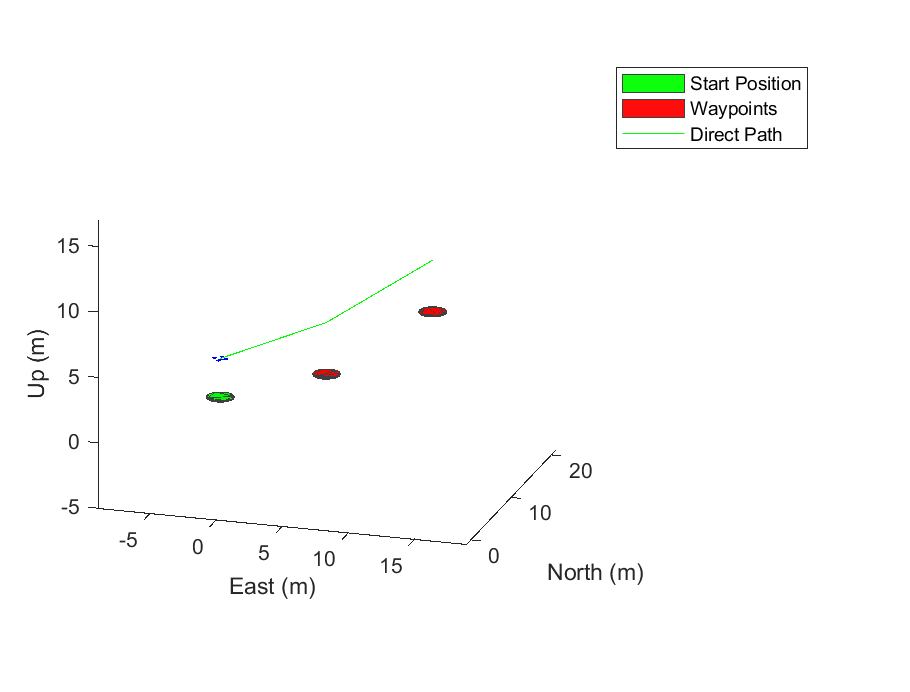
\includegraphics[width = 0.6\textwidth]{./img/3_3_scenario1}
    \caption{Scenario one in open air with no obstacles.}
    \label{fig:3_3_scenario1}
\end{figure}

\subsection{Scenario 2}
The second scenario is shown in Figure \ref{fig:3_3_scenario2}. It consists of two obstacles, with one obstructing the direct path. This scenario aims to test the controller when there is an obstacle involved. It imitates moving between two obstacles, for example two trees. This tests how well the controller can control a change in direction to avoid the obstacle, and the second obstacle serves to prevent excessive turning in this manoeuvre.
\begin{figure}[H]
    \centering
    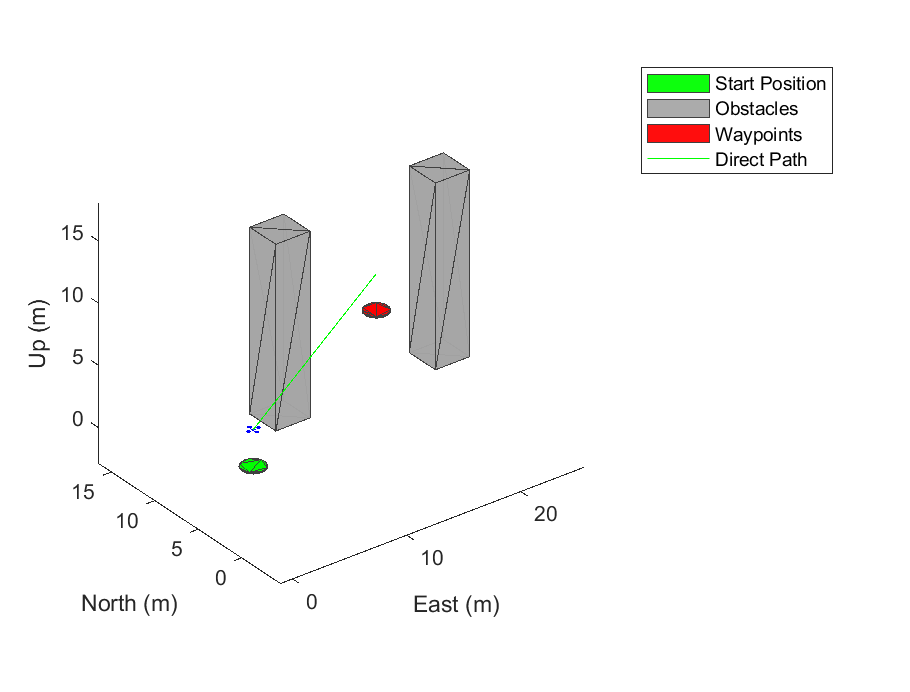
\includegraphics[width = 0.6\textwidth]{./img/3_3_scenario2}
    \caption{Scenario two with a simple obstacle avoidance manoeuvre.}
    \label{fig:3_3_scenario2}
\end{figure}

\subsection{Scenario 3}
The third scenario is shown in Figure \ref{fig:3_3_scenario3}. This scenario is used to test the controller when ascending and descending, to go over an obstacle. This incorporates obstacle avoidance and altitude change to see the movement when the drone senses obstacles beneath it instead of in front of it.
\begin{figure}[H]
    \centering
    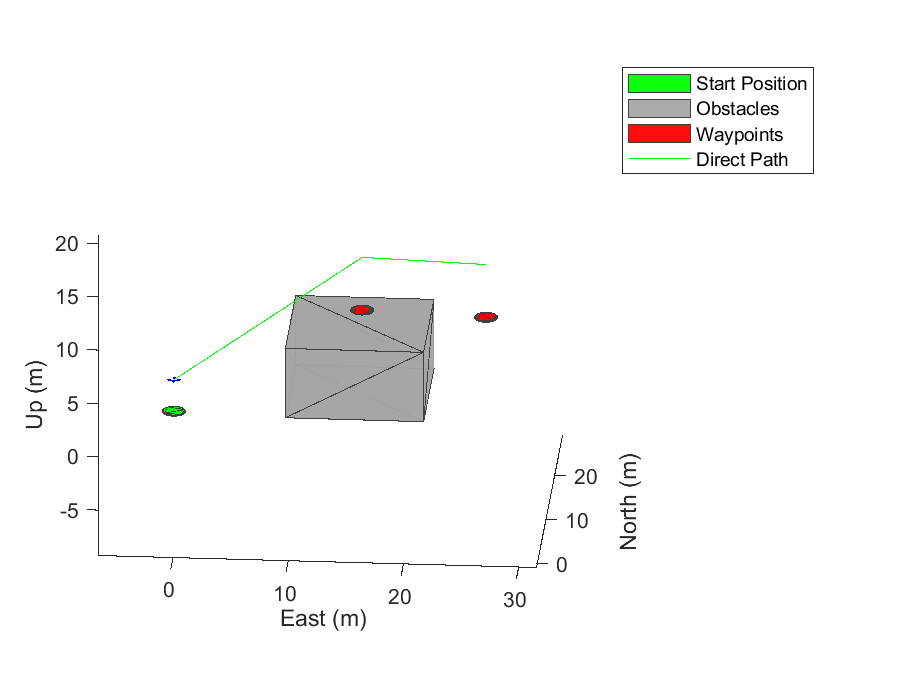
\includegraphics[width = 0.6\textwidth]{./img/3_3_scenario3}
    \caption{Scenario three with a height-varying obstacle avoiding manoeuvre.}
    \label{fig:3_3_scenario3}
\end{figure}

\subsection{Scenario 4}
The fourth scenario is shown in Figure \ref{fig:3_3_scenario4}. This scenario is similar to scenario two, with the addition of an extra waypoint and a change in height of the waypoints. It tests the controller's ability to move around an obstacle, like a pillar or tree. The sharp turn from the first to second waypoint is also another testing point for the controller.
\begin{figure}[H]
    \centering
    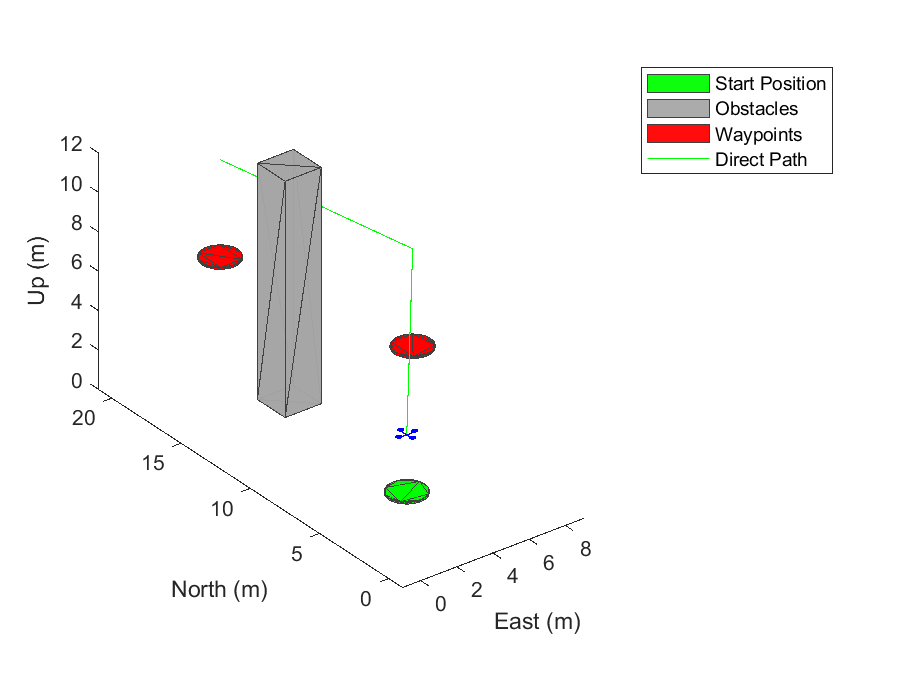
\includegraphics[width = 0.7\textwidth]{./img/3_3_scenario4}
    \caption{Scenario four involves change in height and obstacle avoidance.}
    \label{fig:3_3_scenario4}
\end{figure}

\subsection{Scenario 5}
The fifth scenario is shown in Figure \ref{fig:3_3_scenario5}, the waypoints are all at the same height. This scenario is inspired by urban navigation. It aims to replicate an urban environment, to see the performance of the drone in dense and compact spaces. This is to test movement that involves traversing between obstacles and relatively narrow areas. 
\begin{figure}[H]
    \centering
    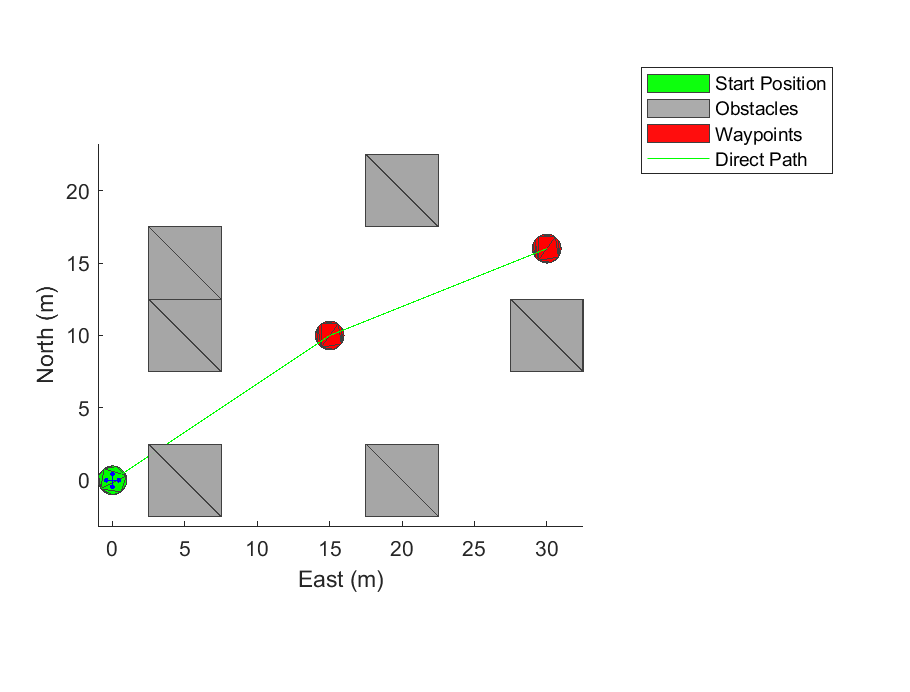
\includegraphics[width = 0.7\textwidth]{./img/3_3_scenario5}
    \caption{Scenario five imitates an urban environment for obstacle avoidance.}
    \label{fig:3_3_scenario5}
\end{figure}